\pdfoutput=1
\documentclass[10pt]{article}
\usepackage[utf8]{inputenc}
\usepackage{arxiv}
\usepackage{orcidlink}
\usepackage{amsmath}
\usepackage{amssymb}
\usepackage{graphicx}
\usepackage{float}
\usepackage{hyperref}
\usepackage[backend=biber, style=apa]{biblatex}
\addbibresource{references.bib}

\title{Universal scale-free representations\\in human visual cortex}

\author{
    \textbf{Raj Magesh Gauthaman$^1$}~\orcidlink{0000-0001-7121-1532},
    \textbf{Brice Ménard$^{2,1,3}$}~\orcidlink{0000-0003-3164-6974},
    \textbf{Michael F. Bonner$^1$}~\orcidlink{0000-0002-4992-674X}\\
    $^1$Department of Cognitive Science,
    $^2$Department of Physics and Astronomy\\
    Johns Hopkins University, Baltimore, MD\\
    $^3$Santa Fe Institute, Santa Fe, NM\\
    \texttt{\{\href{mailto:rgautha1@jh.edu}{rgautha1}, \href{mailto:bmenard1@jh.edu}{bmenard1}, \href{mailto:mfbonner@jh.edu}{mfbonner}\}@jh.edu}
}

\date{}

\begin{document}

\maketitle

\begin{abstract}
    How does the human visual cortex encode sensory information? To
    address this question, we explore the covariance structure of neural
    representations. We perform a cross-decomposition analysis of fMRI
    responses to natural images in multiple individuals from the Natural
    Scenes Dataset and find that neural representations systematically
    exhibit a power-law covariance spectrum over four orders of
    magnitude in ranks. This scale-free structure is found in multiple
    regions along the visual hierarchy, pointing to the existence of a
    generic encoding strategy in visual cortex. We also show that, up to
    a rotation, a large ensemble of principal axes of these population
    codes are shared across subjects, showing the existence of a
    universal high-dimensional representation. This suggests a high
    level of convergence in how the human brain learns to represent
    natural scenes despite individual differences in neuroanatomy and
    experience. We further demonstrate that a spectral approach is
    critical for characterizing population codes in their full extent,
    and in doing so, we reveal a vast space of uncharted dimensions that
    have been out of reach for conventional variance-weighted methods. A
    global view of neural representations thus requires embracing their
    high-dimensional nature and understanding them statistically rather
    than through visual or semantic interpretation of individual
    dimensions.
\end{abstract}

\section{Introduction}\label{introduction}

How does the human visual cortex leverage the activity of large-scale
neural populations to represent sensory information? To what extent are
these visual population codes shared across individuals? Shedding light
on these questions can be done by studying the covariance structure of
neural populations, a quantity describing important aspects of
information processing in neural population activity.

While previous studies have examined the covariance of visual cortex
activity in humans and monkeys, they have largely done so in the service
of dimensionality reduction
\autocite{Khosla2022,Tarhan2020,Haxby2011,Huth2012}. Some of these
studies have argued that dimensionality reduction is implemented by
visual cortex itself to achieve stable representations of behaviorally
relevant information \autocite{Lehky2014,Lehky2016,Fusi2016}. Others
have used dimensionality reduction as a tool to uncover individual
representational dimensions that can be semantically interpreted
\autocite{Thorat2019,Connolly2012,Huth2012,Khosla2022}. Together, these
studies have provided valuable insight into the leading and
highest-variance dimensions of visual cortex activity, but none have
attempted to provide a global characterization of how cortical
populations encode sensory information. To understand the sensory code
in its entirety, we need to go beyond its leading dimensions and examine
stimulus representations at all levels of variance: we need to
characterize its spectrum as broadly as possible.

It is also crucial to understand which aspects of visual cortex
representation are shared across individuals and thus reflect general
properties of human vision. A number of studies have addressed this
question using representational similarity analysis (RSA) and
hyperalignment \autocite{Kriegeskorte2008,Haxby2011,Haxby2020}. However,
these previous studies have not examined the \emph{extent} to which the
underlying dimensions of the cortical sensory code are shared across
individuals. Thus, several fundamental questions remain unanswered. Over
how many dimensions is the shared representation expressed? Do subjects
represent images similarly across all ranks of latent dimensions, or is
the shared code restricted to a core subset of dimensions?

Here we explore the structure of visual neural representations following
a methodological approach closer to physics than traditional
neuroscience. We characterize, as broadly as possible, the spectrum of
representational dimensions that co-vary between trials or subjects. We
do so by leveraging a large-scale dataset of high-resolution fMRI
responses to thousands of natural images \autocite{Allen2021}. Using an
orthogonal cross-decomposition with a generalization test on held-out
images, we show that the covariance spectrum of fMRI responses to
natural images in human visual cortex is consistent with a power-law
distribution over almost four orders of magnitude in latent dimension
ranks. This reveals that the statistics of neural activations are
\emph{scale-free}, a behavior we observe across all individuals and in
multiple visual regions along the cortical hierarchy. Our results are in
line with recent findings of representations with power-law spectra in
the primary visual cortex (V1) of mice\footnote{We will present a
  comparative study of mice and humans in a companion paper.}
\autocite{Stringer2019}. Next, by aligning the activations of different
subjects, we show that they share a common representation over many
latent dimensions, suggesting that they represent the visual world using
a similar scale-free code despite idiosyncrasies in brain anatomy and
learning experiences. In contrast, we find that conventional RSA is only
sensitive to leading, high-variance dimensions and thus fails to reveal
the full extent of these shared population codes. Together, our results
show that human visual cortex represents natural images in cortical
population activity with a universal scale-free spectrum, and they
reveal a rich space of stimulus-related dimensions that have been out of
reach for conventional methods but may be critical for understanding the
cortical code of human vision.

\section{Results}\label{results}

We set out to study the statistical properties of stimulus-related
fluctuations in the fMRI responses of visual cortex and to characterize
the spectral properties of visual representations shared across
individuals. To do so, we analyze the activation covariance, which
captures all second-order (pairwise) interactions between voxels.

An important first step is to characterize the eigenvalue spectrum of
this neural covariance, which describes how variance decays across
dimensions. The spectral decay informs us about the fraction of
dimensions that effectively contribute to the global variance, which is
related to the smoothness of the representation. If the spectrum
displays an exponential decay, this indicates that there is a finite
effective dimensionality capturing most of the variance. In contrast, if
a heavy-tailed distribution is observed, it is necessary to consider the
full spectrum because the effective dimensionality may not have an
intrinsic upper bound other than the total number of neurons, which is
about \(10^9\) in human visual cortex.

Note that it is possible for individuals to have similar covariance
eigenspectra but use different latent dimensions to encode images in
distinct ways. Thus, it is necessary to go beyond characterizing the
spectrum of stimulus-related variance \emph{within} each individual and
identify the degree to which this variance is shared \emph{between}
individuals. By directly examining shared variance, we can identify
representational properties that are consistent across individuals and
are likely to have a fundamental role in visual information processing.

We point out that standard principal component analysis (PCA) of
cortical activations is not adequate to reach our goals as it decomposes
all sources of variance, including both the stimulus-related signal of
interest and noise. In addition, when comparing two individuals, we are
considering two covariances expressed in different spaces, which could
be rotated relative to one another or contain fundamentally different
dimensions. Thus, cross-validation and functional alignment are needed
to identify the shared stimulus-related information in cortical
activity. Below we describe a method to achieve these goals.

\subsection{A spectral method to estimate similarities between
high-dimensional
representations}\label{a-spectral-method-to-estimate-similarities-between-high-dimensional-representations}

Given a pair of subjects \(X\) and \(Y\) who have seen the same images,
we investigate properties of their cortical representation covariances
\(\Sigma_k(X,X)\), \(\Sigma_k(Y,Y)\) and their cross-covariance
\(\Sigma_k(X,Y)\) as a function of rank \(k\) from an orthogonal
decomposition. To estimate the level of similarity between
representations, our goal is to compute the correlation

\begin{equation}\phantomsection\label{eq-correlation-coefficient}{
\mathrm{r}_k(X, Y) =  \frac{\Sigma_k(X,Y)}{\Sigma_k(X,X)^{1/2}\, \Sigma_k(Y,Y)^{1/2}}
}\end{equation}

as a function of rank \(k\) for latent dimensions sorted by decreasing
variance. The correlation function \(r_k\) characterizes the range of
dimensions over which the representation in one subject is shared with
another. For this ratio to be meaningful, it is important to estimate
the numerator and denominator in the same statistical manner and take
into account the following requirements:

\begin{enumerate}
\def\labelenumi{\arabic{enumi}.}
\tightlist
\item
  We want to consider only activations that are stimulus-dependent and
  discard others. This requires cross-validation of covariances using
  repeated stimulus trials. For between-subject comparisons, we average
  over cross-trial comparisons so that the estimator is insensitive to
  the order of the trials.
\item
  To characterize the shared dimensions of different subjects, the
  representations need to be hyperaligned by solving the Procrustes
  problem, which finds the optimal rotation for aligning two matrices
  along shared latent dimensions \autocite{Haxby2011}.
\item
  We are interested in results that generalize and do not reflect chance
  alignments of a particular dataset. To do so, we systematically use
  cross-validated train/test splits in our spectral estimation. This
  cross-validation ensures that if the data are random, the expected
  covariance estimates will be zero rather than being all positive, as
  in a standard orthogonal decomposition.
\end{enumerate}

We refer to this procedure as cross-decomposition. It uses the
orthogonal rotation method from hyperalignment to align representations
along a set of shared latent dimensions \autocite{Haxby2011}. A set of
training data is used to learn these orthogonal transformations. Once
the representations are aligned, we compute cross-validated covariance
estimates along each latent dimension using held-out test data, yielding
a cross-covariance singular value spectrum. In sum, the cross-validated
singular values from this procedure reflect shared stimulus-related
variance that is reliably detected in held-out data. We present a
detailed mathematical formalism of these estimators in the Methods
section. The main steps are also illustrated in
Figure~\ref{fig-schematic}.

We note that while this approach shares similarities with the covariance
eigenspectrum obtained by cross-validated PCA (cvPCA), it also departs
from it in two important ways \autocite{Stringer2019}. First, cvPCA can
only be applied to within-subject analyses. To explore the level of
shared representations between subjects, we need a method that can
meaningfully align their representations. Second, cvPCA examines
reliability across stimulus repetitions for a set of images but does not
examine generalization to new images. Because our goal is to
characterize representational properties that generalize over images,
our cross-decomposition approach assesses both reliability across
stimulus repetitions \emph{and} generalization to new stimuli. As a
result of these differences, cross-decomposition and cvPCA characterize
different statistical quantities whose spectra naturally differ. This is
illustrated in Figure~\ref{fig-schematic}, where standard PCA, cvPCA,
and cross-decomposition exhibit different spectral decays due to their
different generalization requirements. Note that an important
consequence of this is that the power-law slopes observed for different
estimators should not be directly compared.

\begin{figure}

\centering{

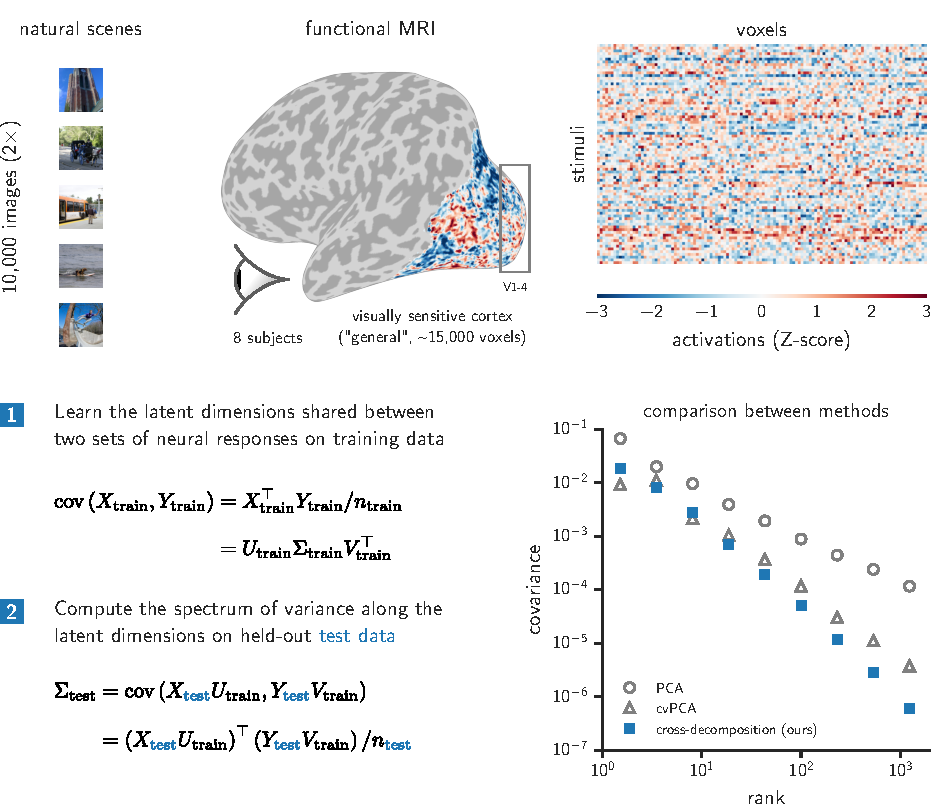
\includegraphics{figures/schematic.pdf}

}

\caption{\label{fig-schematic}\textbf{Cross-decomposition procedure to
estimate the cross-validated spectrum of visual representations.} (Top)
Each participant viewed about \(10,000\) natural scene images multiple
times while their fMRI BOLD responses were measured. The depicted brain
region is a ``general'' region of interest in visual cortex that was
identified by selecting all voxels whose activity was modulated by the
presentation of images. (Bottom) Estimating a cross-validated covariance
spectrum requires identifying directions of variance that are shared
between two sets of cortical responses given a set of training images.
Sets can have repeated presentations of stimuli to a single subject or
repeated presentations of the same stimuli to two different subjects.
The reliable shared variance is then evaluated on cortical responses to
held-out test images. Example spectra are shown for subject 1 based on
our cross-decomposition approach as well as PCA and cvPCA.}

\end{figure}%

Finally, we highlight two important considerations for characterizing
high-dimensional representations:

\begin{enumerate}
\def\labelenumi{\arabic{enumi}.}
\tightlist
\item
  \textbf{A spectral approach} is needed to assess the nature of
  representations in their full extent and to meaningfully compare
  high-dimensional quantities. A spectral approach allows us to to
  determine if representations are localized over a finite range of
  dimensions or spread over an unbounded range (in practice limited by
  the dataset), and it allows us to compare individuals across all
  underlying dimensions of cortical activity. We point out that other
  approaches for comparing representations, such as RSA and centered
  kernel alignment, typically extract a single scalar coefficient of
  similarity that is variance-weighted
  \autocite{Kriegeskorte2008,Kornblith2019}. As a result, they are
  effectively dominated by a relatively limited number of low-rank
  dimensions and are not sensitive to potentially many informative
  high-rank dimensions. We illustrate this point in
  Figure~\ref{fig-rsa}, which is discussed in detail in
  Section~\ref{sec-similarity-of-scale-free-representations}. To explore
  high-dimensional properties of neural representations, it is necessary
  to take a spectral approach and estimate quantities as a function of
  rank \(k\) obtained from an orthogonal decomposition. As described in
  Equation~\ref{eq-correlation-coefficient}, our goal is therefore to
  estimate a correlation function \(r_k\) rather than a single scalar
  coefficient.
\item
  \textbf{Aggregating latent dimensions} by binning the statistical
  estimates in our spectra can provide substantial gains in sensitivity,
  allowing us to measure spectral shape well beyond the range over which
  individual components are detected. This comes at the cost of lowering
  the resolution at which we characterize the latent space of the
  system, but, if the spectrum presents a smooth dependence on rank,
  this aggregation can reduce noise with a negligible loss of
  information. Such an approach is ubiquitous in physics. In contrast,
  previous work in neuroscience has often focused on latent dimensions
  that can be individually detected (and, if possible, interpreted).
  When focusing on individual dimensions, the unavoidable presence of
  noise imposes severe limitations on the range of dimensions that can
  be studied and effectively limits such an approach to a
  low-dimensional view of neural representation. Here, our goal is to
  probe the statistical structure of activation covariances and
  characterize the full extent of the spectrum of visual representations
  and their similarities between individuals.
\end{enumerate}

\subsection{Scale-free representations in visual
cortex}\label{scale-free-representations-in-visual-cortex}

We first used our cross-decomposition approach to characterize, as
broadly as possible, the spectrum of image representations in a general
region of interest (ROI), including all visually responsive voxels. The
results are presented in the left panel of Figure~\ref{fig-general}.
Interestingly, despite focusing on only stimulus-related variance that
generalizes to held-out data (i.e., putting strong requirements on the
selected variance), we can reliably detect signals following a power-law
distribution across four orders of magnitude of latent dimensions. As
described in the methods section, we normalized the overall amplitude of
covariances to account for the varying number of voxels between
individuals (see Figure~\ref{fig-vary-n-voxels}). The error bars in
Figure~\ref{fig-general} depict variance across cross-validation folds,
demonstrating that the covariance statistics are reliably estimated.
Furthermore, in Figure~\ref{fig-significance-test}, we performed
permutation tests by randomly shuffling images before computing the
covariance estimates, allowing us to further demonstrate that the
observed covariance spectrum is statistically significant over a wide
range of ranks.

These findings have several key implications. First, they demonstrate
that human visual cortex represents natural images in population
activity that is \emph{scale-free}. The scale-free nature of these
representations implies that their dimensionality is ill-defined:
estimates of effective dimensionality for visual cortex likely reflect
the properties of a given dataset (i.e., the number and richness of
stimuli, the number of recording channels) rather than an intrinsic
property of cortical representation. In fact, our findings suggest that
the representations of visual cortex are expressed over \emph{all}
available dimensions and that, given the power-law behavior, any
low-rank truncation of these representations would lead to a
non-negligible loss of stimulus-related information. Given that the
maximum reachable rank is commensurate with the number of neurons in
visual cortex, the neglected information could be immense. Second, the
observed consistency of these spectra across subjects shows that there
is universality in how variance is spread across latent dimensions in
different individuals. In other words, visual cortex representations
have the same level of smoothness across people.

\begin{figure}

\centering{

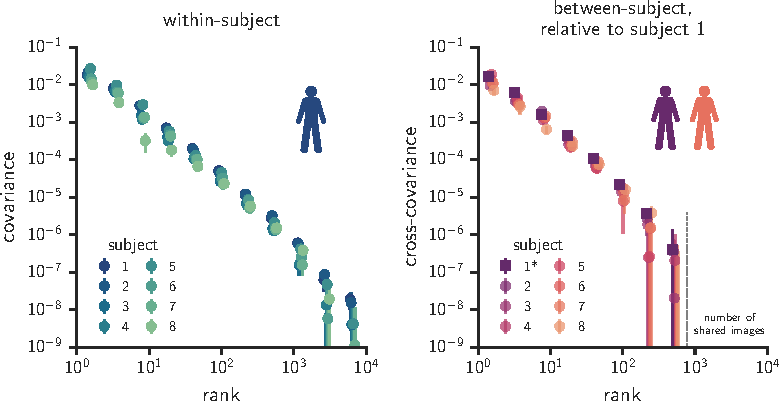
\includegraphics{figures/general.pdf}

}

\caption{\label{fig-general}\textbf{Cortical representations of natural
images are scale-free and shared across subjects over many dimensions.}
(Left) Within-subject covariance spectra of visual cortex responses in a
general region of interest including all visually responsive voxels from
the Natural Scenes fMRI dataset \autocite{Allen2021}. (Right)
Between-subject covariance spectra for the same region of interest,
characterizing shared variance relative to reference subject 1. The
range is limited by the number of shared stimuli seen by all subjects.
All spectra are normalized to account for differences in the number of
voxels across participants and averaged within bins of exponentially
increasing width and across 8 folds of cross-validation. Error bars
denote standard deviations across these 8 folds.
Figure~\ref{fig-general-all} shows the results of the same analysis
using each subject as the reference subject.}

\end{figure}%

We also observed that the typical spatial scales over which fMRI signals
fluctuate decrease with rank. This is illustrated in
Figure~\ref{fig-singular-vectors}. This suggests that the scale-free
property of cortical representations exists over a wide range of
physical scales, from tens of centimeters down to the limiting
resolution of the experiment (i.e., 1.8 mm). Interestingly, similar
scale-free covariance spectra have been reported in the primary visual
cortex of the mouse brain \autocite{Stringer2019}. These results are
based on calcium imaging measurements of individual neurons (i.e., on
physical scales several orders of magnitude smaller than the ones used
in our fMRI analysis). Together, our findings and the previous findings
in mice point to a possible ubiquity of scale-free activation spectra in
mammalian visual cortex. Note that, as mentioned above, the power-law
exponents of the mouse spectra from \textcite{Stringer2019} and the
human spectra reported here cannot be directly compared, as they are
based on different statistical estimators. In a companion paper, we will
present direct quantitative comparisons of the spectra in humans and
mice.

In summary, our results show that visual cortex representations are
expressed over several orders of magnitude of latent dimensions and
display a universal scale-free spectrum. While the variance is dominated
by a subspace substantially smaller than the entire space, the
scale-free nature of the spectrum suggests that its dimensionality is
ill-defined and likely unbounded (up to the number of neurons).

\subsection{A representational code shared across
individuals}\label{a-representational-code-shared-across-individuals}

We next explore whether representational dimensions are shared
\emph{between} individuals (i.e., whether their latent dimensions
co-vary for the same stimuli). Representations can be compared across
subjects using methods like RSA \autocite{Kriegeskorte2008} or
hyperalignment \autocite{Haxby2011}, with the latter enabling
comparisons of individual dimensions across subjects. This
hyperalignment is achieved by our cross-decomposition technique. We use
it to estimate the cross-covariance spectrum between individuals
\(\Sigma_k(X,Y)\) for the available subset of approximately 1,000 images
which were shown to all participants in the Natural Scenes Dataset
experiment.

The right panel of Figure~\ref{fig-general} shows the results for
comparisons relative to subject 1. In this figure, the square symbols
represent the within-subject spectrum for subject 1 (as in the left
panel), and the circles represent comparisons with other subjects. This
analysis reveals that the between-subject spectra are remarkably similar
to the within-subject spectrum---again exhibiting a scale-free power-law
distribution that spans nearly three orders of magnitude of latent
dimensions. Comparisons between all other pairs of subjects yielded
similar results and are shown in Figure~\ref{fig-general-all}.
Permutation tests again showed that the observed covariance spectra are
robustly detected across many ranks
(Figure~\ref{fig-significance-test}). Note that the upper bounds of
these spectra are limited by the size of the available dataset---we
expect that with more stimuli, even more shared dimensions would likely
be revealed.

As shown in Figure~\ref{fig-cross-detectability}, if we rely on
anatomical alignment alone and assume that subject-specific rotations
are irrelevant, we only detect shared variance up to about ten
dimensions. Thus, while these dimensions may have similar coarse-scale
anatomical properties across individuals, shared dimensions at higher
ranks require subject-specific functional alignment to be detected.

In sum, these results show that visual representations co-vary between
subjects over many ranks of dimensions, and they suggest that despite
differences in experience and cortical anatomy, the visual cortices of
different individuals converge to a universal scale-free code for
natural image representation.

\begin{figure}

\centering{

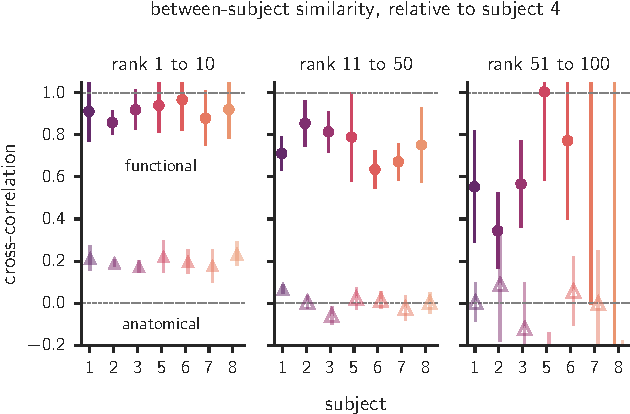
\includegraphics{figures/cross-correlations.pdf}

}

\caption{\label{fig-cross-correlations}\textbf{Representational
similarity in visual cortex for pairs of subjects.} Correlation of
neural representations as a function of ranks obtained from the ratio of
cross-validated between-subject variance relative to cross-validated
within-subject variance (Equation~\ref{eq-correlation-coefficient}).
These findings show that the stimulus-related variance in cortical
activity is largely shared across subjects over many ranks. Furthermore,
the similarity of high-rank dimensions can only be detected when the
representations are functionally aligned in a shared space using
subject-specific rotation matrices. With anatomical alignment alone,
shared representations are undetectable beyond \(\approx 10\)
dimensions. Error bars denote standard deviations across 8 folds of
cross-validation. Open symbols denote points where the mean is less than
three standard deviations above zero.
Figure~\ref{fig-cross-correlations-all} shows the results of the same
analysis using each subject as the reference subject.}

\end{figure}%

\subsection{Similarity of scale-free
representations}\label{sec-similarity-of-scale-free-representations}

We next address a central question about the nature of shared
representations: To what degree are neural representations shared
between individuals? Having performed spectral decomposition of both the
within-subject and between-subject covariances, we can now compare the
ratio of these covariance estimates to determine the proportion of
stimulus-related variance that is shared between individuals.
Specifically, we compute the set of correlation coefficients
\(\mathrm{r}_k(X,Y)\) between subjects as a function of rank
(Equation~\ref{eq-correlation-coefficient}). Being ratios, these
correlation coefficients are expected to be noisier than the
corresponding covariance spectra. To ensure a sufficiently high
signal-to-noise, we aggregated these ratios over wider bins of ranks
than used above.

As shown in Figure~\ref{fig-cross-correlations}, our analysis reveals a
high level of correlation over a range of latent dimensions, a finding
that is consistent for all subjects considered in the analysis. While we
can only detect the correlations among subjects over two orders of
magnitude in ranks, our observation of universal power-law distributions
in both the within-subject and between-subject spectra suggests that
this correlation likely holds well beyond this range
(Figure~\ref{fig-general}). This prediction can be tested in the future
with larger datasets. It is also worth noting that while these plots
show a remarkable degree of similarity across subjects, some level of
subject-specific stimulus-related variance gradually emerges with ranks.
An intriguing question for future work is to investigate whether this
subject-specific variance reflects meaningful individual differences in
visual processing and to determine whether individual differences
reliably increase as a function of latent-dimension rank.

As mentioned above, our cross-decomposition approach together with a
spectral analysis were critical for revealing the high-dimensional
nature of these shared representations. Specifically, to meaningfully
compare population activity between subjects, it is necessary to
\emph{functionally} align their representations into a shared space by
applying hyperlignment (i.e., subject-specific rotation matrices)
\autocite{Haxby2011}. If we use anatomical alignment alone and assume
that subject-specific rotation matrices are not needed, we only detect
representational similarity for the first ten dimensions, as shown by
the triangle symbols in Figure~\ref{fig-cross-correlations}. In
addition, it is important to note that variance-weighted estimators
(without any spectral decomposition) are mainly sensitive to low-rank
dimensions and therefore not adequate to probe the properties of
high-dimensional representations. We found that a conventional
implementation of RSA is effectively sensitive to only a handful of
latent dimensions and cannot distinguish between low- and
high-dimensional representations, as demonstrated in
Figure~\ref{fig-rsa}. Furthermore, visualizations show that the low-rank
dimensions detected with anatomical alignment and RSA correspond to
coarse-scale gradients of cortical tuning, as shown in
Figure~\ref{fig-singular-vectors}. Thus, the conventional methods of
cognitive neuroscience provide a view of neural representation that is
effectively low-dimensional and spatially coarse.

\begin{figure}

\centering{

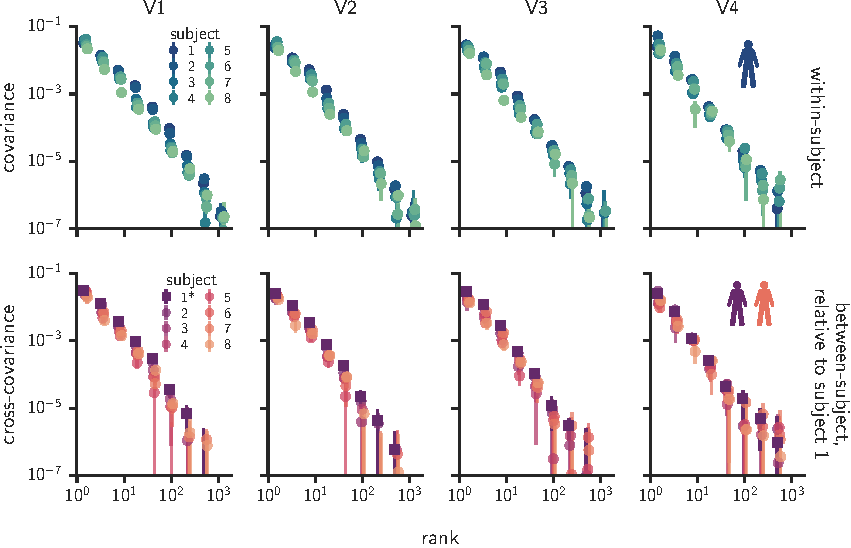
\includegraphics{figures/v1-to-v4.pdf}

}

\caption{\label{fig-v1-to-v4}\textbf{Scale-free representations are
consistently observed across multiple regions of visual cortex.} These
plots show within-subject (top) and between-subject (bottom) covariance
spectra for retinotopic regions along the visual hierarchy from V1 to
V4. In comparison with the larger region of interest shown in
Figure~\ref{fig-general}, these findings demonstrate that the same
scale-free power-law distribution is observed in smaller regions of
interest, and they show that these power-law distributions are highly
consistent across regions. This implies that across these regions of the
visual hierarchy, there is universality in the smoothness of cortical
population codes. Further, the between-subject spectra show that each of
these regions represents images using high-dimensional codes that are
shared across individuals. Error bars denote standard deviations across
8 folds of cross-validation.}

\end{figure}%

In sum, these findings show that the stimulus representations of visual
cortex are not only scale-free but also encode similar information in
the brains of different individuals. Most of these representational
dimensions have subject-specific anatomical properties, making them
undetectable with anatomical alignment alone, and they are obscured in
the representational similarity matrices of RSA---functional alignment
and spectral analyses are necessary for revealing these shared
dimensions. The shared nature of these representations implies that the
entire spectrum of activity contributes to the sensory code. This
suggests that there is a wealth of representational content in
measurements of visual cortex that has remained beyond the reach of
conventional methods but may be crucial for understanding human vision.

\subsection{Consistent behavior across visual cortex
regions}\label{consistent-behavior-across-visual-cortex-regions}

After first focusing on a large and general ROI of visually responsive
voxels, we next investigate whether our findings are representative of
the structure of population codes observed across different visual
regions. To answer this question, we computed both the within- and
between-subject cross-decomposition spectra for the retinotopic regions
V1, V2, V3, and V4. As shown in Figure~\ref{fig-v1-to-v4}, we found the
spectra in these regions to be highly similar to the spectra observed
for the general ROI, despite these retinotopic ROIs being much smaller
in size. This is observed for both the within-subject and
between-subject cross-decomposition analyses. This finding suggests that
there is spatial-scale invariance in the power-law spectrum of visual
cortex activity: a consistent power law is observed when considering a
large general ROI of all visually responsive voxels or when considering
much smaller retinotopic ROIs. Furthermore, these findings show that the
spectra are highly consistent across regions, which means that we do not
find evidence for either dimensionality reduction or expansion along
consecutive stages of visual processing. Thus, at least up to mid-level
visual regions (i.e., V4), the representations of visual cortex exhibit
a universal scale-free format with a characteristic power-law index.

\section{Discussion}\label{discussion}

\subsection{The nature of neural
representations}\label{the-nature-of-neural-representations}

\subsubsection{Key results}\label{key-results}

We found that the population codes of human visual cortex are scale-free
and, to a great extent, shared among individuals. Scale-free cortical
activity patterns represent sensory information using the full range of
their latent dimensions, and this sensory information is largely shared
across subjects. Due to their scale-free nature, these representations
cannot be reduced without discarding reliable sensory signal and
attempts to quantify their effective dimensionality depend on the size
of the dataset. We observe stimulus-related variance to decay across the
principal axes of these population codes according to a characteristic
power-law distribution. The same power law was observed in all subjects,
in multiple regions along the visual hierarchy, and at multiple spatial
scales, which suggests that there is a fixed balance between the
contributions of low- and high-rank dimensions in the cortical code for
vision. In short, these findings reveal a universal scale-free
representation of natural scenes in the human brain.

Though many previous studies have examined visual representations in
human and monkeys through the lens of dimensionality reduction
\autocites[e.g.][]{Lehky2014,Khosla2022}, recent results obtained from
calcium imaging of the mouse brain have revealed scale-free power-law
distributions over at least two decades of ranks in the cross-validated
covariance spectra of cortical populations
\autocite{Stringer2019,Manley2024}. The specific power-law exponents
from these studies and ours cannot be compared directly due to
differences in statistical estimators (as illustrated in
Figure~\ref{fig-schematic}). We will present direct quantitative
comparisons of the mouse and human spectra in a companion paper.
Nonetheless, these studies in mice and our work in humans demonstrate
convergent findings of scale-free structure in cortical activity
patterns measured at vastly different spatial resolutions, and they
suggest that scale-free population codes may be a general
representational strategy of mammalian cerebral cortex.

\subsubsection{Implications for neural
mechanisms}\label{implications-for-neural-mechanisms}

The observation of a consistent spectral behavior across individuals,
brain regions, spatial scales, and possibly species is a strong
indication that a simple, generic neural mechanism is at play, likely to
arise from principles of network self-organization. It is important to
understand its nature as it speaks to the fundamental principles that
govern the activity and computations of neural populations. Previous
work suggests several possible hypotheses, which are not mutually
exclusive. It has been proposed that power-law covariance eigenspectra
emerge in neural populations that strike an optimal balance between
expressivity and robustness \autocite{Stringer2019}. Along these lines,
\textcite{Prince2024} showed that when the covariance eigenspectra of
artificial neural networks are made to achieve this balance through
regularization during learning, they exhibit a better representational
match to human visual cortex. Using connectivity arguments,
\textcite{Lynn2024} showed that a Hebbian learning mechanism yields
heavy-tailed neuronal connectivity distributions which, under certain
conditions, may lead to scale-free covariance spectra. One appeal of
such a Hebbian learning account is that it does not require
goal-directed feedback (i.e., backpropagation). An exciting direction
for future work is to identify which principles govern the underlying
mechanism leading to the scale-free representations of mammalian
cerebral cortex.

Previous work has argued that the level of dimensionality in a brain
region is linked to the region's functional specialization, with some
functions calling for high dimensionality and others low dimensionality
\autocites[e.g.][]{Fusi2016,CaycoGajic2019}. In the case of vision,
there have been conflicting proposals about the link between
dimensionality and visual information processing. Some have argued for
the importance of dimensionality \emph{expansion} to improve linear
separability of stimulus classes \autocite{Elmoznino2024,Babadi2014}.
Others have argued for the importance of dimensionality \emph{reduction}
to suppress irrelevant variance and yield robust representations of
behaviorally relevant variables
\autocite{Ansuini2019,Cohen2020,Lehky2016,Fusi2016}. However, our
findings suggest that natural image representations neither expand nor
contract along successive stages of the visual hierarchy, at least up to
mid-level representations. Instead, we observe a remarkable degree of
stability in the power-law structure of visual population codes. An
important question for future work is whether differences in
dimensionality may emerge in downstream regions that support
higher-level visual cognition.

Prior investigations have shown that visual cortex representations are
at least partly shared across people and species
\autocite{Haxby2011,Kriegeskorte2008} and that hyperalignment is
critical for uncovering the common dimensions that underlie these shared
representations \autocite{Haxby2011,Haxby2020}. Our work pushes this
exploration further by showing that the shared representations are
scale-free: they are expressed over all dimensions and only limited by
the size of the data. Furthermore, we quantified the portion of
stimulus-related variance within each subject that is shared with
others, and we found that, remarkably, this variance is shared over a
wide range of ranks. This means that across the range considered in this
analysis, images are represented in a similar way in the brains of
different individuals. Thus, despite differences in experience and brain
anatomy, the human visual system appears to converge to a common
high-dimensional code for natural images.

As in previous work \autocite{Haxby2011}, our findings show that the
shared representational dimensions of different brains can only be fully
observed by hyperaligning the cortical activity patterns from one
individual to another. This implies that the underlying dimensions of
the representational code are not spatially localized but instead
correspond to latent dimensions that are distributed. Although the brain
clearly exhibits spatially localized functions on large scales (e.g.,
the visual cortex is well localized), our results indicate that when
examining brain activity on progressively smaller scales, the
representations become more distributed. Indeed, we only found evidence
for shared spatial localization in the first decade of the
representational spectrum, with the bulk of stimulus-related information
expressed through universal latent dimensions that have distinct spatial
distributions in each subject and require subject-specific rotation
matrices. An important goal for future work is to understand what kind
of learning mechanism can explain how the human brain converges to a
shared representational code over many dimensions despite
subject-specific spatial organization. Some insight might come from
studies of artificial neural networks, which also exhibit universal
learning properties that can be detected in their latent dimensions
rather than their neurons \autocites[e.g.][]{Guth2024,Chen2024}.

\subsubsection{Limitations of our
analysis}\label{limitations-of-our-analysis}

In this work, we explored the properties of neural representations using
linear methods, based on an orthogonal decomposition of variance in all
directions, with a generalization test in held-out data. This linear
description of activations is appealing as it characterizes the
information that could be decoded by downstream neurons implementing a
simple linear readout procedure, which is a key motivation for the
usefulness of this approach. However, it is possible that nonlinear
mappings of representations could provide lower-dimensional descriptions
of visual cortex activity \autocite{Ansuini2019,De2023,Jazayeri2021}. If
so, the shared representation between individuals could potentially be
an intrinsically lower dimensional object. An exciting direction for
future work is the pursuit of cross-validated nonlinear dimensionality
methods that can allow for direct comparisons of linear and nonlinear
dimensionality measurements of stimulus-dependent variance.

\subsection{Comments on traditional approaches in cognitive
neuroscience}\label{comments-on-traditional-approaches-in-cognitive-neuroscience}

\subsubsection{The ``low-resolution'' view of variance-weighted
estimators in
neuroscience}\label{the-low-resolution-view-of-variance-weighted-estimators-in-neuroscience}

The scale-free nature of sensory representations observed here has
important implications for the methods of neuroscience. First, it is a
common practice to examine neural representations through dimensionality
reduction
\autocite{Cunningham2014,Huth2012,Haxby2011,Khosla2022,Lehky2014}. In
such approaches, researchers typically invoke a criterion to identify a
subset of ``signal'' dimensions that account for much of the variance in
the data, while discarding the remaining dimensions, which are
considered either unimportant or noise-dominated. However, a robust
estimate of the covariance spectrum reveals a power-law distribution
rather than a distribution with an exponential cutoff. This implies that
there is no intrinsic upper bound on the ``signal'' dimensions, and it
suggests that while typical dimensionality-reduction methods may account
for much of the \emph{variance}, they discard much of the
\emph{information}, which can be found in the long tail of low-variance
but nonetheless reliable dimensions. Another important implication is
that typical \emph{variance-weighted} estimators, including RSA,
voxelwise encoding models (i.e., regression), and linear classifiers,
are insensitive to the full extent of information in a power-law
distribution. Instead, these methods exhibit a sensitivity to latent
dimensions that decays rapidly with rank and becomes vanishingly small
beyond the first decade of ranked dimensions. Thus, the correlation
metrics obtained with these methods are unable to fully capture the
richness of representations expressed in high dimensions. We demonstrate
this point in Figure~\ref{fig-rsa} by presenting RSA analyses of
representations in low and high dimensions, which show that this
technique is effectively insensitive to the effects from ranks greater
than about \(10\). Moreover, because low-rank dimensions correspond to
large-scale cortical gradients, this means that typical
variance-weighted methods, like RSA, effectively view neural
representations through a spatially low-resolution lens. This suggests
that there is a vast space of uncharted dimensions in neural activity
that has been out of reach for conventional methods and whose role in
human cognition has yet to be thoroughly investigated.

\subsubsection{Limitations of brain maps and semantic
interpretations}\label{limitations-of-brain-maps-and-semantic-interpretations}

Another consideration raised by our findings is that common methods used
for visualizing and interpreting neural representations are severely
limited in their ability to characterize high-dimensional information.
One such method is brain mapping, which cognitive and systems
neuroscientists use to characterize the spatial organization of response
preferences to representational dimensions
\autocite{Huth2012,Bao2020,Tarhan2020,Hebart2023,Contier2024}. One brain
map can only convey a small number of representational dimensions.
However, as we have shown, human brain representations are expressed
using the full dimensionality of the available space (ultimately defined
by the number of neurons) and through a scale-free activation spectrum.
An unrealistic number of brain maps would be needed to convey the robust
high-dimensional sensory information that our spectral analysis reveals.
As a result, brain map visualizations can only scratch the surface of
neural representations and cannot illuminate the full extent of the
reliable information in cortical population activity. Furthermore,
because of the need to hyperalign subjects to find their shared
dimensions, the common approach of averaging fMRI results over
anatomically aligned brains effectively limits our view to the
relatively small number of dimensions whose anatomical distributions are
highly similar across subjects. We suggest that understanding neural
representations in their entirety requires a transition from a
localized, map-based view of the brain to a more distributed statistical
description that considers the full spectrum of the cortical code.

A similar consideration applies to the semantic interpretation of
representational dimensions, which is typically restricted to low-rank
dimensions that can be individually detected without the need for
spectral binning \autocite{Huth2012,Khosla2022,Tarhan2020,Hebart2023}.
As we showed, aggregating dimensions allows one to dramatically extend
the range over which latent dimensions are detectable. Such a binning
procedure, though common in other fields that examine power-law
distributions \autocite{Lin2023}, has not typically been used in studies
of neural representation. Doing so requires that we focus on the
spectrum as a whole rather than seeking to interpret each latent
dimension. Intriguingly, scale-free properties can be found in multiple
aspects of the brain, as previous studies have detected scale-free
power-law distributions in temporal activity patterns, structural
connectivity, and behavior \autocite{He2014,Lynn2024,Kello2010}. This
suggests that methods for rigorously characterizing phenomena
distributed over many orders of magnitude may prove crucial to
understanding the human brain. To be clear, we believe that the
visualization methods of previous work have revealed important
organizing properties of the brain. However, if we want to move beyond
low-dimensional characterizations of neural representation, we need to
embrace approaches for exploring representations in their full extent
and understanding them mathematically rather than visually or
semantically \autocite{Roads2024}.

\subsection{Summary}\label{summary}

Together, our findings reveal the scale-free format of the cortical code
for human vision. We found that natural images evoke reliable variance
with a power-law spectrum across multiple orders of magnitude of latent
dimensions. Importantly, we also found that a large number of these
dimensions are shared across individuals, suggesting a remarkable degree
of convergence despite individual differences in neuroanatomy and
experience. To obtain a global view that captures more than the first
\(\sim 10\) dimensions, it is crucial to use both spectral analysis and
functional alignment. Otherwise, one is typically limited to
high-variance dimensions (as is the case for RSA) or the subset of
dimensions that tend to be anatomically aligned. In sum, these findings
suggest that the sensory code of visual cortex spans all available
dimensions of population activity and that fully understanding human
brain representations requires a high-dimensional statistical approach.

\newpage{}

\section{Methods}\label{methods}

\subsection{Dataset}\label{dataset}

\subsubsection{Experimental design}\label{experimental-design}

We used the Natural Scenes Dataset (NSD), a large-scale 7T fMRI dataset
of image-evoked blood-oxygen-level-dependent (BOLD) responses to
approximately 10,000 stimuli in each of eight participants. The stimuli
were taken from the Common Objects in Context (COCO) image dataset, and
they contain photographs of a large and diverse set of objects in their
natural scene contexts. Participants viewed these images in the scanner
while performing a recognition memory task (i.e., ``Have you seen this
image before?''). Images were shown three times over the course of the
experiment, and trial-level response estimates were obtained for
\(\sim 30,000\) stimulus presentations (about 10,000 images \(\times\) 3
trials per image). A subset of 1,000 images were seen by all
participants in the experiment while the remaining images were unique to
each participant. However, note that some participants did not complete
all scan sessions and, thus, had fewer stimulus trials.

\subsubsection{Data preprocessing}\label{data-preprocessing}

We used the 1.8 mm volumetric preparation of the data, with version b2
of the betas (betas\_fithrf), which were z-scored within each scanning
session to reduce non-stationarity, as recommended by the authors. We
refrained from using the denoised version b3 of the betas
(betas\_fithrf\_GLMdenoiseRR) since (i) the dimensionality reduction
applied by the denoising might remove reliable low-variance signal and
(ii) these betas were specifically optimized to maximize reliability
across trials, which could bias our analyses of reliable cross-trial
variance.

\subsubsection{Regions of interest}\label{regions-of-interest}

For our main analyses, we focused on a pre-defined ``general'' region of
interest (ROI), which included all stimulus-responsive voxels in visual
cortex (i.e., the large ``nsdgeneral'' ROI ranging in size from 12,000
to 18,000 voxels across subjects). We also performed follow-up analyses
in smaller ROIs (i.e., the retinotopic regions V1, V2, V3, and V4) to
explore possible changes along the visual processing stream.

\subsection{Formalism}\label{formalism}

Given the representations of \(n\) stimuli in two different systems, the
neural responses can be organized into two data matrices
\(X \in \mathbb{R}^{n \times d_X}\) and
\(Y \in \mathbb{R}^{n \times d_Y}\) where the rows correspond to \(n\)
presented stimuli and the \(d_X, d_Y\) columns correspond to the numbers
of recording channels --- here, voxels from functional neuroimaging. Our
goal is to characterize the similarities between the representations of
two neural systems. We do so by characterizing their neural
representation covariances \(\Sigma_k(X, X)\) and \(\Sigma_k(Y, Y)\) and
the cross-covariance \(\Sigma_k(X, Y)\) as a function of rank \(k\) from
an orthogonal decomposition. The similarity can then be quantified by
the spectral correlation

\[
\mathrm{r}_k(X, Y) =  \frac{\Sigma_k(X, Y)}{\Sigma_k(X, X)^{1/2}\, \Sigma_k(Y, Y)^{1/2}}\;.
\]

\subsection{\texorpdfstring{Computing within-subject spectra
\(\Sigma_k(X, X)\)}{Computing within-subject spectra \textbackslash Sigma\_k(X, X)}}\label{computing-within-subject-spectra-sigma_kx-x}

To robustly estimate the covariance spectrum \(\Sigma_k\) of neural
responses to stimuli, we compute the cross-covariance of neural
responses to the same images on different trials, say \(X_1\) and
\(X_2\), which ensures that the estimated covariance generalizes across
repeated presentations of the stimuli. Additionally, we cross-validate
the covariance spectra across images to ensure that we extract
stimulus-related variance and not stimulus-independent noise.

Specifically, we split \(X\) into \emph{training} and \emph{test} sets
\(X_\text{train}\) and \(X_\text{test}\), compute the singular value
decomposition of the cross-covariance of the training data

\[
\operatorname{cov}
\left(X_{1,\text{train}} , X_{2,\text{train}}\right)
= n^{-1}\,X_{1,\text{train}}^\top\,X_{2,\text{train}}
= U_\text{train}\, \Sigma_\text{train}\, V_\text{train}^\top
\]

and evaluate the reliable variance along each latent dimension by
projecting the test data onto the singular vectors \(U_\text{train}\)
and \(V_\text{train}\)

\[
\Sigma(X_1, X_2) = \operatorname{cov}
\left(X_{\text{1,test}}\,U_\text{train}, X_{\text{2,test}}\,V_\text{train} \right) / d_X
\]

where the normalization by \(d_X\) (number of voxels) enables meaningful
comparisons between representations with different numbers of channels
(see Figure~\ref{fig-vary-n-voxels} for more detail). All the data are
centered using the mean of the training sets.

When the train and test samples are drawn from the same distribution,
the covariance matrix \(\Sigma\) is diagonal in expectation. In
practice, under normal circumstances, \(\Sigma\) is quasi-diagonal and
we have verified that the contribution from off-diagonal terms is
negligible. We thus estimate the cross-validated spectrum as

\[
\hat{\Sigma}_k(X, X) = \mathrm{diagonal~of~}\Sigma(X_1, X_2)\;.
\]

\subsubsection{Cross-validation scheme}\label{cross-validation-scheme}

To use all available data, we divide the stimuli into 8 folds, then use
7 folds to learn singular vectors and the remaining fold to estimate
variance along the dimensions. Specifically, \(X_\text{train}\) has 7
times as many stimuli as \(X_\text{test}\). We repeat this process 8
times using each fold as the test set once, producing eight spectra.
Finally, we average the binned spectra across all 8 folds to obtain
\(\hat{\Sigma}_k\).

\subsection{\texorpdfstring{Computing between-subject spectra
\(\Sigma_k(X,Y)\)}{Computing between-subject spectra \textbackslash Sigma\_k(X,Y)}}\label{computing-between-subject-spectra-sigma_kxy}

When computing \emph{between-subject} spectra, \(X_i\) contains neural
responses from subject \(X\) on the \(i\)\textsuperscript{th}
presentation of the shared stimuli while \(Y_j\) contains neural
responses from subject \(Y\) on the \(j\)\textsuperscript{th}
presentation of the shared stimuli.

We compute the singular value decomposition of the cross-covariance
between the two training sets of neural responses

\[
\operatorname{cov}
\left(X_{i,\text{train}} , Y_{j,\text{train}}\right)
= n^{-1}\,X_{i,\text{train}}^\top\,Y_{j,\text{train}}
= U_\text{train}\, \Sigma_\text{train}\, V_\text{train}^\top
\]

and evaluate the covariance that generalizes to held-out stimuli by
projecting the test sets onto the singular vectors \(U_\text{train}\)
and \(V_\text{train}\)

\[
\hat{\Sigma}_k(X_i,Y_j) = \mathrm{diagonal~of~} \operatorname{cov}
\left(X_{i, \text{test}}\, U_\text{train} , Y_{j, \text{test}}\, V_\text{train} \right) / \sqrt{d_X d_Y}
\]

where the normalization by the geometric mean of the number of voxels
\(d_X\) and \(d_Y\) enables meaningful comparisons between the spectra
for different pairs of subjects.

Since the ordering of trials is arbitrary, we make the estimated
spectrum symmetric by averaging the spectra for two pairs of trials: (i)
\(X_1\) and \(Y_2\) and (ii) \(X_2\) and \(Y_1\), making our final
estimate of the spectrum

\[
\hat{\Sigma}_k(X,Y) = \frac{1}{2}\left[\hat{\Sigma}_k(X_1,Y_2) + \hat{\Sigma}_k(X_2,Y_1)\right]\;.
\]

Similar to our procedure for the within-subject spectra, we divide the
stimuli into 8 folds and estimate cross-validated binned spectra.

Note that for all of these spectral analyses, the test singular values
\(\hat{\Sigma}_k(X, X)\) and \(\hat{\Sigma}_k(X, Y)\) are not guaranteed
to be positive, unlike a typical singular value spectrum. In fact, if
the two systems share no reliable covariance that generalizes from the
training set to the test set along a particular singular vector, the
expected value of the corresponding test singular value is \(0\). We
make use of this property to perform the null test shown in the inset of
Figure~\ref{fig-significance-test}.

\subsubsection{Functional vs anatomical
alignment}\label{functional-vs-anatomical-alignment}

In the lower panels of Figure~\ref{fig-general}, we refer to the
between-subject spectra described above as \emph{functionally} aligned
spectra since they are computed by decomposing a cross-covariance matrix
that assumes no anatomical alignment between the voxels across
individuals. If we assume that different subjects' cortical surfaces are
in fact anatomically aligned, i.e.~the voxels at the same location in
different subjects have identical tuning properties, we would expect
that the latent dimensions from one participant should generalize to
another. Specifically, we would expect that the rotation matrices
\(U_\text{train}\) and \(V_\text{train}\) corresponding to the first and
second subjects respectively could be swapped without losing any
information when estimating cross-validated covariance on the test data.

We thus compute \emph{anatomical} spectra by projecting
\(X_\text{test}\) onto \(V_\text{train}\) instead of \(U_\text{train}\)
and \(Y_\text{test}\) onto \(U_\text{train}\) instead of
\(V_\text{train}\) and computing the covariance of the resulting
projections. Since this procedure requires that the columns
\(U_\text{train}\) and \(V_\text{train}\) correspond to the same
anatomically aligned voxels across both subjects, we map all the neural
responses onto the standard Montreal Neurological Institute (MNI) space,
downsample them to isotropic 1.8 mm voxels that match the resolution of
the original dataset, and restrict our analyses to the common voxels
that are present in both individuals. Both the \emph{functional} and
\emph{anatomical} spectra are computed on these data to ensure that they
are directly comparable.

\subsection{Representational similarity
analyses}\label{representational-similarity-analyses}

Representational similarity matrices (RSMs) were constructed for each
subject by computing Pearson correlations between patterns of fMRI
responses to pairs of images and repeating this for all image pairs
(using single trial-level responses from the ``nsdgeneral'' region of
interest for each image, exactly as in the between-subject
cross-decomposition analyses shown in the right panel of
Figure~\ref{fig-general}). RSA correlations were obtained by correlating
the RSMs for two subjects using either the linear (Pearson) or
rank-order (Spearman) correlation coefficient. This procedure reflects a
standard approach for comparing the representations of two individuals
or an individual and a model. It is representative of a broader class of
variance-weighted similarity metrics that also includes regression-based
encoding models \autocite{Kriegeskorte2019,Kornblith2019}.

\subsubsection{Code availability}\label{code-availability}

All code for these analyses are available at
\href{https://github.com/BonnerLab/scale-free-visual-cortex}{this git
repository}.

\section{Acknowledgments}\label{acknowledgments}

This research was supported in part by a Johns Hopkins Catalyst Award to
MFB, Institute for Data Intensive Engineering and Science Seed Funding
to MFB and BM, and grant NSF PHY-2309135 to the Kavli Institute for
Theoretical Physics.

\newpage{}

\section*{Supplementary Figures}\label{supplementary-figures}
\addcontentsline{toc}{section}{Supplementary Figures}

\setcounter{figure}{0}
\counterwithin{figure}{section}
\renewcommand{\thefigure}{S\arabic{figure}}

\begin{figure}[H]

\centering{

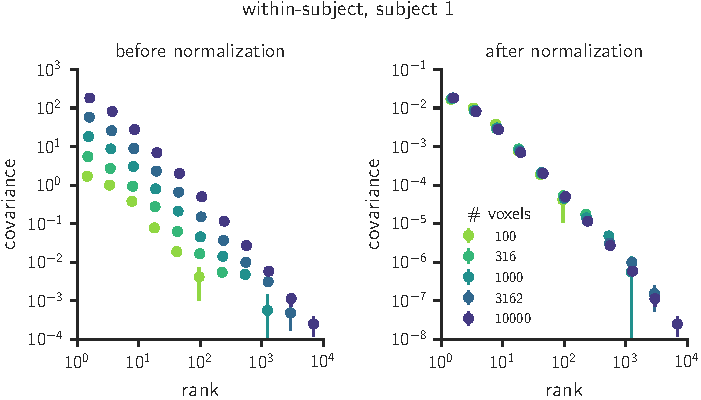
\includegraphics{figures/vary-n-voxels.pdf}

}

\caption{\label{fig-vary-n-voxels}\textbf{Spectral normalization} (Left)
Within-subject cross-trial spectra were computed with different numbers
of voxels sampled from the general region of interest. Increasing the
number of voxels leads to higher variance. (Right) Normalizing the
spectra by the number of voxels accounts for these differences.}

\end{figure}%

\begin{figure}[H]

\centering{

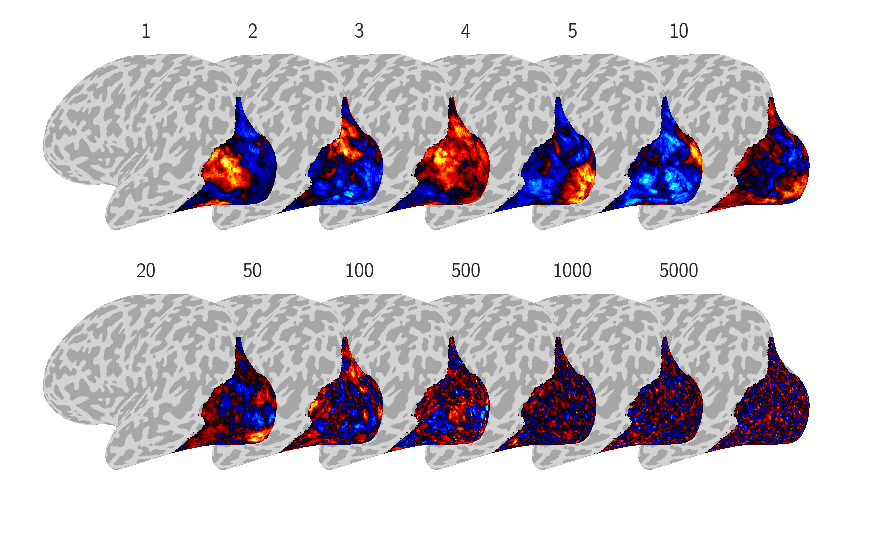
\includegraphics{figures/singular-vectors.pdf}

}

\caption{\label{fig-singular-vectors}\textbf{Examples of singular
vectors as a function of rank} obtained from our within-subject
cross-decomposition analysis for subject 1 displayed on the cortical
surface. The typical spatial scale decreases monotonically with ranks.}

\end{figure}%

\begin{figure}[H]

\centering{

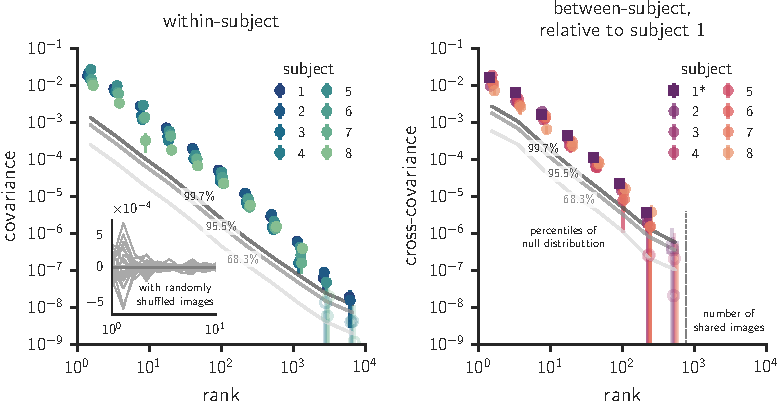
\includegraphics{figures/significance-test.pdf}

}

\caption{\label{fig-significance-test}\textbf{Within- and
between-subject covariance spectra compared to null tests.} This plot
displays the same results as Figure~\ref{fig-general} with gray contours
indicating the 68\textsuperscript{th}, 95\textsuperscript{th} and
99\textsuperscript{th} percentiles of null distributions obtained by
randomly shuffling images before computing the covariance estimates
(\(n = 5,000\) permutations). Ten samples of this null distribution are
displayed in the inset, illustrating that the spectra have an expected
value of zero when no reliable covariance is shared between the two
datasets. Open symbols denote points that are not significant at
\(p < 0.001\). This permutation test shows good agreement with the error
bars denoting the standard deviations across 8 different splits of the
data.}

\end{figure}%

\begin{figure}[H]

\centering{

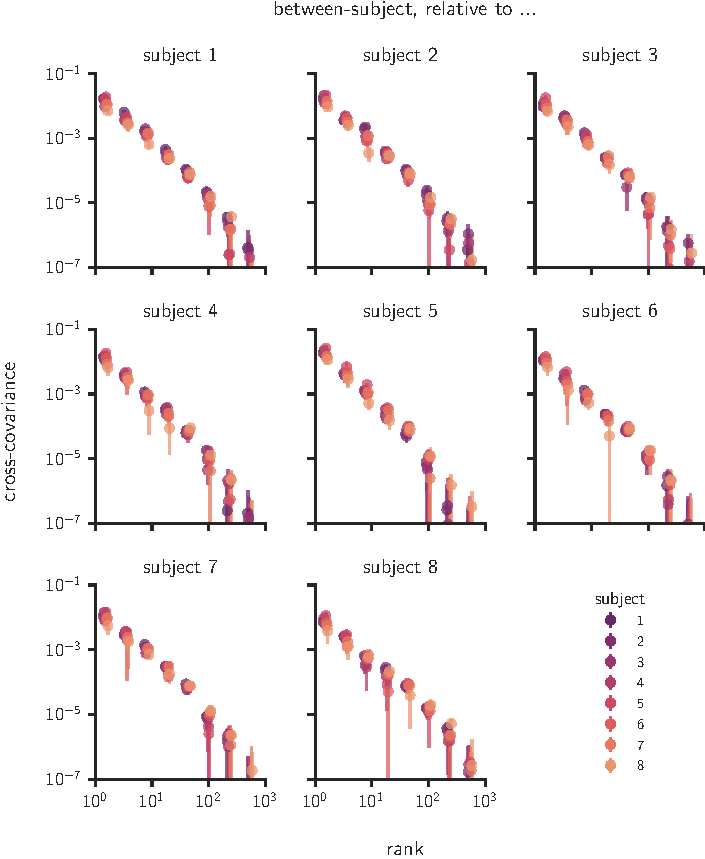
\includegraphics{figures/general-all.pdf}

}

\caption{\label{fig-general-all}\textbf{Between-subject covariance
spectra in the general visual region, relative to each subject.} These
plots show the same analysis as in the upper right panel of
Figure~\ref{fig-general} but with each subject treated as the reference
subject.}

\end{figure}%

\begin{figure}[H]

\centering{

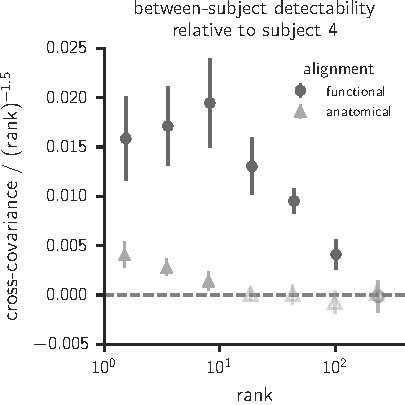
\includegraphics{figures/cross-detectability.pdf}

}

\caption{\label{fig-cross-detectability}\textbf{Comparison between
cross-spectra obtained using functional and anatomical alignment,
relative to a reference subject 1.} The two measured spectra are
normalized by a power law to visualize their behavior over multiple
orders of magnitude. While anatomically alignment reveals only
\(\approx 10\) shared latent dimensions, functionally aligning subjects
reveals many more shared latent dimensions. Open symbols denote points
where the mean is less than three standard deviations above zero.}

\end{figure}%

\begin{figure}[H]

\centering{

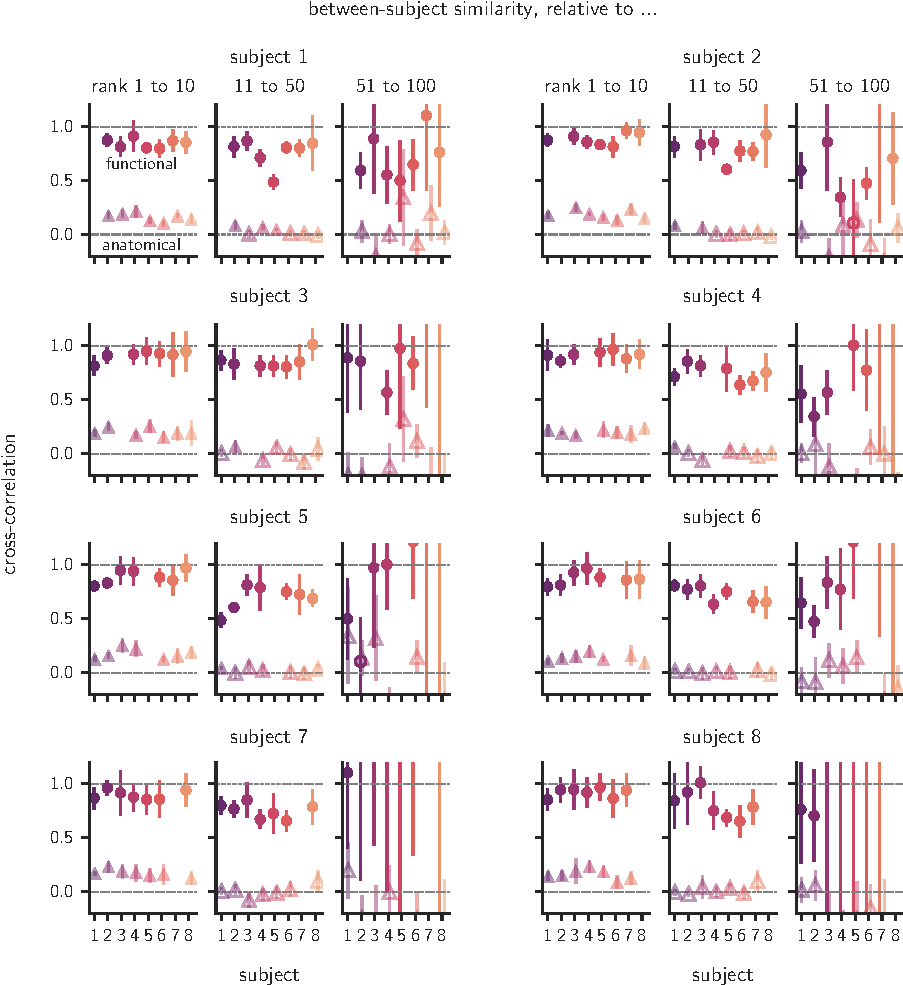
\includegraphics{figures/cross-correlations-all.pdf}

}

\caption{\label{fig-cross-correlations-all}\textbf{Representational
similarity in visual cortex for all pairs of subjects.} These plot shows
the same analysis as in Figure~\ref{fig-cross-correlations} but with
each subject treated as the reference subject.}

\end{figure}%

\begin{figure}[H]

\centering{

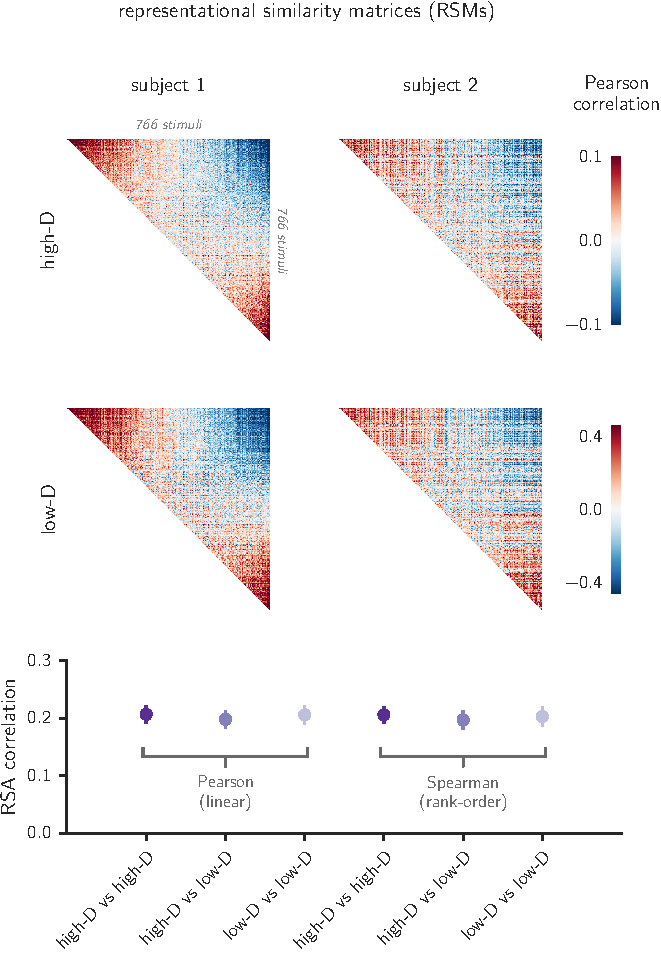
\includegraphics{figures/rsa.pdf}

}

\caption{\label{fig-rsa}\textbf{RSA correlations are largely insensitive
to high-dimensional structure.} Representational similarity analysis
(RSA) was used to compare the visual cortex representations of two
individuals. (Top) This analysis was performed on two sets of RSMs: one
computed on the original fMRI data (``high-D'') and a second computed on
reduced-rank fMRI data (``low-D''). Reduced-rank fMRI data was generated
by applying principal component analysis to the fMRI response matrices
and then reconstructing each matrix from its first \(10\) principal
components (PCs). As can be seen by the RSM visualizations, this
dimension-reduction procedure has little effect on the RSMs because the
underlying similarity metrics are largely driven by the leading PCs of
the response matrices. (Bottom) The mean RSA correlation across all
pairs of subjects remains nearly identical even after the data for one
subject in each pair has been drastically reduced to just \(10\) PCs
(compare ``high-D vs high-D'' to ``high-D vs low-D''). The same
phenomenon is observed when computing RSA scores using both linear
Pearson correlations (left) and rank-order Spearman correlations. These
results illustrate that variance-weighted similarity metrics, which are
dominated by the leading PCs of neural activity, are effectively
insensitive to the shared variance at high-rank dimensions that can be
detected with our cross-decomposition approach, which extends well
beyond \(10\) ranks (Figure~\ref{fig-general}). Error bars denote 2
standard deviations across 5,000 bootstrap samples. For each bootstrap
sample, 90\% of the stimuli were subsampled without repetition before
computing representational similarity matrices (RSMs).}

\end{figure}%

\newpage
\printbibliography

\end{document}
